\documentclass[10pt,twoside]{report}
\linespread{1.19} 

\usepackage[dvipsnames]{xcolor}
\usepackage[export]{adjustbox}
\usepackage[utf8]{inputenc}
\usepackage{graphicx}
\graphicspath{ {images/} }
\usepackage{float}

\usepackage[a4paper,width=150mm,top=25mm,bottom=25mm,bindingoffset=6mm]{geometry}
\usepackage{caption}
\usepackage{subcaption}
\usepackage[hidelinks]{hyperref}
\usepackage{float}
\usepackage{fancyhdr}
\pagestyle{fancy}

\usepackage{amssymb}
\usepackage{amsmath}
\usepackage[linesnumbered,ruled,vlined]{algorithm2e} 
\usepackage{tikz}
\usetikzlibrary{shadings, patterns}
\usepackage{enumitem}
\usepackage{array}

% Custom column types
\newcolumntype{L}[1]{>{\raggedright\arraybackslash}p{#1}} % Left-aligned fixed width
\newcolumntype{C}[1]{>{\centering\arraybackslash}p{#1}}   % Center-aligned fixed width
\newcolumntype{R}[1]{>{\raggedleft\arraybackslash}p{#1}}  % Right-aligned fixed width

\usepackage{tikz}
\usetikzlibrary{shapes.geometric, arrows}
\tikzstyle{startstop} = [rectangle, rounded corners, minimum width=3cm, minimum height=1cm, text width=3cm,text centered, draw=black, fill=blue!30]
\tikzstyle{io} = [trapezium, trapezium left angle=70, trapezium right angle=110, minimum width=3cm, minimum height=1cm, text width=3cm, text centered, draw=black, fill=blue!30]
\tikzstyle{process} = [rectangle, minimum width=3cm, minimum height=1cm, text width=3cm, text centered, draw=black, fill=orange!30]
\tikzstyle{decision} = [diamond, minimum width=3cm, minimum height=1cm, text centered, draw=black, fill=green!30]
\tikzstyle{mux} = [rectangle,text width=0.1cm, draw=black, fill=black]
\tikzstyle{arrow} = [thick, text width=3cm,text centered,->,>=stealth]

\usepackage{listings} % for code insertion
\definecolor{codegreen}{rgb}{0,0.6,0}
\definecolor{codegray}{rgb}{0.5,0.5,0.5}
\definecolor{codepurple}{rgb}{0.58,0,0.82}
\definecolor{backcolour}{rgb}{0.95,0.95,0.92}

\lstdefinestyle{mystyle}{
    backgroundcolor=\color{backcolour},   
    commentstyle=\color{codegreen},
    keywordstyle=\color{magenta},
    numberstyle=\tiny\color{codegray},
    stringstyle=\color{codepurple},
    basicstyle=\ttfamily\footnotesize,
    breakatwhitespace=false,         
    breaklines=true,                 
    captionpos=b,                    
    keepspaces=true,                 
    numbers=left,                    
    numbersep=5pt,                  
    showspaces=false,                
    showstringspaces=false,
    showtabs=false,                  
    tabsize=2
}

\lstset{style=mystyle}

\title{

% \textbf{DynoCharge Business Plan}

{\huge \textbf{BUSSINESS PLAN}}\\
\vspace{0.5cm}
{
\large
{\huge\textbf{DynoCharge}}\\
}\\
\vspace{0.3cm}
\vspace{0.5cm}
\textbf{Victor Ezea}

\vspace{0.6cm}
\vspace{0.6cm}
\textbf{Contact Information:} \\
Victor Ezea \\
ezeavictorchukwuebuka@gmail.com \\
+33758942230 \\
4D Boulevard de la Gare, Boissy Saint Ledger, 94470, France
}

\date{10, March 2025}


\begin{document}

\maketitle

\pagenumbering{gobble}
\pagestyle{empty}
\tableofcontents
\clearpage
\pagestyle{plain}

\listoffigures
\listoftables


\pagenumbering{arabic}

% Executive Summary
\section{1. Executive Summary}
DynoCharge is a European electric vehicle (EV) charging startup deploying ultra-fast (150kW+), smart, and sustainable charging stations to address Europe’s critical EV infrastructure gaps. By integrating renewable energy partnerships and advanced software, we aim to make EV charging as convenient as traditional refueling while driving the transition to zero-emission mobility.

\subsection*{Vision}
To become Europe’s most trusted and accessible EV charging network by 2030, enabling seamless, emission-free travel across urban and rural regions.

\subsection*{Mission}
Deliver reliable, affordable, and ultra-fast charging solutions for EV drivers, fleets, and businesses while advancing Europe’s renewable energy adoption.

\subsection*{Key Metrics (Year 1 Goals)}
\begin{table}[h!]
    \centering
    \renewcommand{\arraystretch}{1.5}
    \begin{tabular}{|>{\bfseries}m{0.4\textwidth}|m{0.5\textwidth}|}
    \hline
    \textbf{Metric} & \textbf{Target} \\
    \hline
    Charging Stations Deployed & 150 \\
    \hline
    Active Users & 10,000 \\
    \hline
    Revenue & €800,000 \\
    \hline
    Charger Uptime & 99\% \\
    \hline
    Customer Satisfaction & 4.7/5 \\
    \hline
    \end{tabular}
    \caption{Year 1 Goals}
\end{table}


% Company Overview

\section{2. Company Overview}
DynoCharge operates as a full-service EV charging provider with a vertically integrated model:

\subsection*{Core Offerings}

\textbf{Hardware:}
\begin{itemize}
    \item 150kW+ DC Fast Chargers with dual ports (CCS/CHAdeMO), battery storage, and solar integration.
    \item \textit{Smart Grid Compatibility:} Bidirectional charging to support grid stability.
\end{itemize}

\textbf{Software:}
\begin{itemize}
    \item Proprietary app with real-time station availability, dynamic pricing, and energy management.
    \item Integration with Apple Pay, Google Pay, and fleet management systems (e.g., Samsara).
\end{itemize}

\textbf{Maintenance:}
\begin{itemize}
    \item \textit{24/7 Monitoring:} AI-driven predictive maintenance to minimize downtime.
    \item \textit{Rapid-Response Teams:} $<$2-hour repair SLA in urban areas, $<$4 hours in rural zones.
\end{itemize}

\subsection*{Industry Overview}
\begin{itemize}
\item \textbf{Market Growth:} Europe’s EV market is growing at 40\% CAGR (2023--2030), with 12 million EVs expected by 2025.

\item \textbf{Policy Drivers:} EU’s ``Fit for 55'' mandates a 55\% CO\textsubscript{2} reduction by 2030, with €800M allocated for charging infrastructure.

\item \textbf{Infrastructure Gap:} Only 330,000 public chargers exist today vs. the 1 million required by 2025 (ACEA).
\end{itemize}

% Problem and Solution
\section{3. Problem and Solution}

\subsection*{Problems}
\begin{itemize}
    \item \textbf{Charging Deserts:} 60\% of rural EU regions lack public chargers, stifling EV adoption.
    \item \textbf{Slow Charging:} 70\% of existing chargers operate below 50kW, requiring 1+ hours for a full charge.
    \item \textbf{Fragmented Networks:} Drivers use 5+ apps to navigate competing providers.
\end{itemize}

\subsection*{Solutions}
\textbf{Ultra-Fast Chargers:}
\begin{itemize}
    \item 150kW+ Stations reduce charging time to 20--30 minutes (vs. 1+ hours for 50kW chargers).
    \item \textit{Battery Buffering:} On-site batteries ensure consistent power delivery during peak demand.
\end{itemize}

\textbf{Strategic Coverage:}
\begin{itemize}
    \item 50\% of Stations deployed in underserved rural areas (e.g., Andalusia, Bavaria).
    \item \textit{Urban Hubs:} Partnerships with shopping malls (e.g., Carrefour) for high-traffic locations.
\end{itemize}

\textbf{Unified Platform:}
\begin{itemize}
    \item Single app for payments, route planning, and energy optimization.
    \item \textit{Fleet API:} Custom dashboards for logistics companies to monitor charging costs in real time.
\end{itemize}


% Target Market

\section {Target Market}

\begin{tabular}{|l|l|l|}
\hline
\textbf{Segment} & \textbf{Pain Points} & \textbf{DynoCharge Solution} \\
\hline
\textbf{EV Owners} & Long wait times, unreliable networks & Fast charging, 99\% uptime, app integration \\
\hline
\textbf{Fleet Operators} & High operational costs, downtime & Bulk pricing, dedicated support, fleet API \\
\hline
\textbf{Municipalities} & Meeting CO2 targets, budget constraints & Revenue-sharing model, solar integration \\
\hline
\textbf{Businesses} & Employee retention, sustainability goals & Workplace charging, branded stations \\
\hline
\end{tabular}




% Market Size & Segments

\section{5. Market Size \& Segments}
\textbf{Market Overview:}  
Europe’s EV charging market will grow to €15.6B by 2027 (Statista).

\subsection*{Key Segments}
\begin{itemize}
    \item\textbf{Public Charging (70\%):}
    \begin{itemize}
        \item\textit{Highway Corridors:} 30\% of demand (e.g., France’s A6 motorway).
        \item \textit{Urban Hubs:} 40\% of demand (shopping centers, office complexes).
    \end{itemize}
    \item \textbf{Residential (20\%):} Home installations for urban EV owners.
    \item \textbf{Fleet (10\%):} Custom depots for delivery/logistics companies (e.g., DHL).
\end{itemize}
\subsection*{Regional Focus (Year 1)}
\begin{table}[h!]
    \centering
    \renewcommand{\arraystretch}{1.5}
    \begin{tabular}{|>{\bfseries}m{0.25\textwidth}|m{0.15\textwidth}|m{0.5\textwidth}|}
    \hline
    \textbf{Country} & \textbf{Chargers} & \textbf{Strategy} \\
    \hline
    France & 60 & Rural regions (Brittany), highway partnerships \\
    \hline
    Germany & 45 & Urban hubs (Berlin, Munich), fleet contracts \\
    \hline
    Spain & 45 & Tourist routes (Costa del Sol), solar-powered stations \\
    \hline
    \end{tabular}
    \caption{Regional Focus and Strategy for Year 1}
\end{table}


% Competition
\section{6. Competition}

\subsection*{Competitor Analysis}
\begin{table}[h!]
    \centering
    \renewcommand{\arraystretch}{1.5}
    \begin{tabular}{|>{\bfseries}m{0.2\textwidth}|m{0.25\textwidth}|m{0.25\textwidth}|m{0.25\textwidth}|}
    \hline
    \textbf{Competitor} & \textbf{Strengths} & \textbf{Weaknesses} & \textbf{DynoCharge Edge} \\
    \hline
    Ionity & 350kW chargers, highway dominance & High prices (€0.43/kWh), no rural coverage & 20\% lower pricing, rural focus \\
    \hline
    Shell Recharge & Brand recognition, 50k+ stations & Slow chargers (50kW), no renewables & 3x faster charging, solar integration \\
    \hline
    Tesla & Exclusive network, loyalty & Closed ecosystem, limited compatibility & Open to all EVs, unified app \\
    \hline
    \end{tabular}
    \caption{Competitor Analysis}
\end{table}

\subsection*{Market Share (2024)}
\begin{itemize}
    \item Tesla: 25\%
    \item Shell Recharge: 20\%
    \item Ionity: 15\%
    \item Others: 40\%
\end{itemize}

\subsection{Market Share of Competitors}
\begin{figure}[h!]
    \centering
    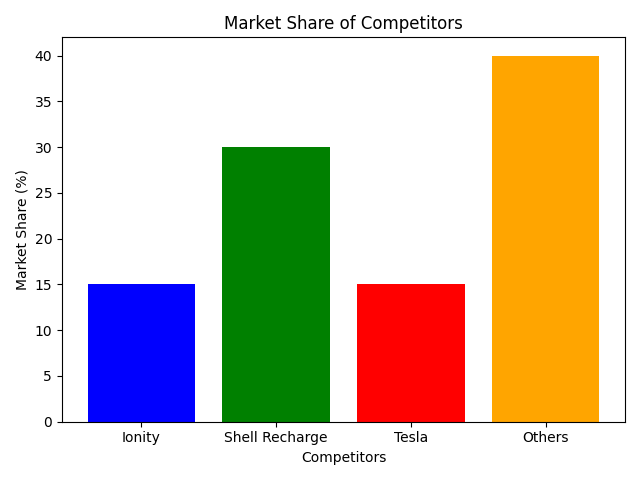
\includegraphics[width=0.8\textwidth]{images/Marketshare.png}
    \caption{Market share of competitors in the EV charging industry.}
    \label{fig:market_share}
\end{figure}


% Competitive Advantages
\section{7. Competitive Advantages}

\subsection*{Technology Leadership}
\begin{itemize}
    \item 150kW+ Chargers with solar/battery integration (30\% energy from renewables).
    \item Predictive Maintenance: AI reduces downtime to <1\% vs. industry average of 5\%.
\end{itemize}

\subsection*{Strategic Partnerships}
\begin{itemize}
    \item E.ON \& Ørsted: 100\% renewable energy supply.
    \item Renault/Nissan: Co-branded stations at dealerships.
\end{itemize}

\subsection*{Pricing Model}
\begin{itemize}
    \item €0.35/kWh (vs. Ionity’s €0.43).
\end{itemize}

\subsection*{Fleet Discounts}
\begin{itemize}
    \item Volume pricing at €0.30/kWh for 100+ EVs.
\end{itemize}


% Product or Service Offerings

\section{8. Product or Service Offerings}

DynoCharge provides a range of EV charging solutions designed for speed, reliability, and sustainability:

\subsection*{Ultra-Fast Charger}
\begin{itemize}
    \item 150kW+ power, dual ports (CCS/CHAdeMO), solar-ready.
    \item \textbf{€50,000/unit} (includes installation).
\end{itemize}

\subsection*{Pricing Table}
\begin{table}[h!]
    \centering
    \renewcommand{\arraystretch}{1.5}
    \begin{tabular}{|>{\bfseries}m{0.2\textwidth}|m{0.45\textwidth}|m{0.2\textwidth}|}
    \hline
    \textbf{Product} & \textbf{Key Features} & \textbf{Pricing} \\
    \hline
    Ultra-Fast Charger & 150kW+, solar-ready, dual ports & €50,000/unit \\
    \hline
    Home Charger & 22kW wallbox, app-controlled & €1,500 installed \\
    \hline
    Fleet Package & Custom depots, API integration & €10k/month (10+ EVs) \\
    \hline
    Maintenance Services & 24/7 monitoring, <2hr response & €200/station/month \\
    \hline
    \end{tabular}
    \caption{Pricing and Features for DynoCharge Products}
\end{table}

\subsection*{Product Details}

\subsubsection*{Home Charger}
\begin{itemize}
    \item 22kW wallbox, app-controlled, compact design.
    \item \textbf{€1,500} (installed, 2-year warranty).
\end{itemize}

\subsubsection*{Fleet Package}
\begin{itemize}
    \item Custom depots, API integration, bulk pricing (€0.30/kWh for 100+ EVs).
    \item \textbf{€10,000/month} (10+ EVs, includes maintenance).
\end{itemize}

\subsubsection*{Maintenance Services}
\begin{itemize}
    \item 24/7 monitoring, <2hr response, 99\% uptime.
    \item \textbf{€200/station/month}.
\end{itemize}

\subsection*{Why DynoCharge?}
\begin{itemize}
    \item \textbf{Fast:} 20–30 minute charging.
    \item \textbf{Sustainable:} Solar integration, renewable energy.
    \item \textbf{Reliable:} 99\% uptime, rapid maintenance.
    \item \textbf{Flexible:} Solutions for individuals, businesses, and fleets.
\end{itemize}


% Marketing Plan
\section{9. Marketing Plan}

\subsection*{Budget Allocation (€150,000)}

\begin{itemize}
    \item \textbf{Digital Ads (40\%):}
    \begin{itemize}
        \item Google Ads targeting “EV charging near me.”
        \item LinkedIn campaigns for fleet operators.
    \end{itemize}
    \item \textbf{Partnerships (30\%):}
    \begin{itemize}
        \item Co-marketing with automakers (Renault, VW).
        \item Free charging weekends at partnered malls.
    \end{itemize}
    \item \textbf{Content (20\%):}
    \begin{itemize}
        \item YouTube tutorials (“How to charge in 20 mins”).
        \item Blog series on sustainability (e.g., “Solar + EVs = Zero Emissions”).
    \end{itemize}
    \item \textbf{Events (10\%):}
    \begin{itemize}
        \item Sponsorship of EU Green Mobility Summit.
    \end{itemize}
\end{itemize}

\subsection*{KPIs}
\begin{itemize}
    \item 5,000 app downloads (Q1).
    \item 20\% conversion rate from free to paid users.
    \item 15+ municipal contracts (e.g., Barcelona, Lyon).
\end{itemize}

\subsection{Marketing Budget Allocation}
\begin{figure}[h!]
    \centering
    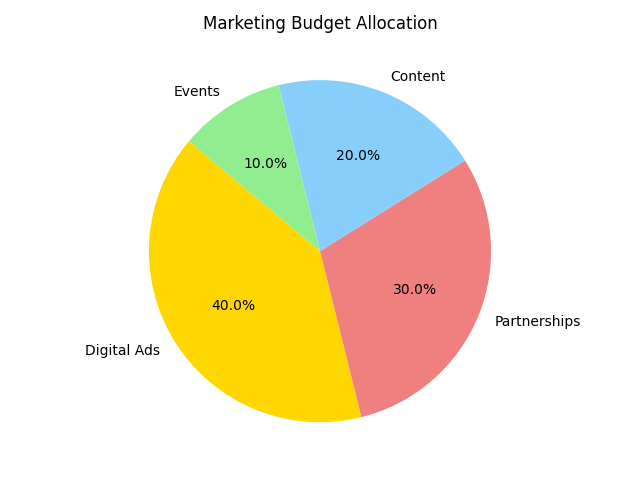
\includegraphics[width=0.8\textwidth]{images/Market budget allogation.png}
    \caption{Marketing budget allocation across digital ads, partnerships, content, and events.}
    \label{fig:marketing_budget}
\end{figure}


% Timeline & Metrics
\section{10. Timeline \& Metrics}

\subsection*{Year 1 Roadmap}

\subsubsection*{Q1: Market Entry}
\begin{itemize}
    \item \textbf{Milestones:} Deploy 50 chargers; onboard 2,000 users.
    \item \textbf{Revenue Target:} €100k (pay-per-use, subscriptions).
\end{itemize}

\subsubsection*{Q2: Expansion}
\begin{itemize}
    \item \textbf{Milestones:} Expand to Germany; secure 3 fleet contracts.
    \item \textbf{Revenue Target:} €250k (fleet deals, growing user base).
\end{itemize}

\subsubsection*{Q3: Sustainability Push}
\begin{itemize}
    \item \textbf{Milestones:} Deploy 50 solar-powered stations; reach 7,000 users.
    \item \textbf{Revenue Target:} €400k (solar stations, subscriptions).
\end{itemize}

\subsubsection*{Q4: Scale \& Profitability}
\begin{itemize}
    \item \textbf{Milestones:} Achieve 10,000 users; break-even.
    \item \textbf{Revenue Target:} €800k (diversified revenue streams).
\end{itemize}

\subsection*{Quarterly Overview}
\begin{tabular}{|c|c|c|}
\hline
\textbf{Quarter} & \textbf{Key Milestones} & \textbf{Financial Target} \\
\hline
Q1 & Launch 50 chargers; onboard 2,000 users & €100,000 revenue \\
Q2 & Expand to Germany; secure 3 fleet contracts & €250,000 revenue \\
Q3 & Install 50 solar-powered stations & €400,000 revenue \\
Q4 & Reach 10,000 users; break-even & €800,000 revenue \\
\hline
\end{tabular}

\noindent



% Financial Forecasts
\section{11. Financial Forecasts}

\subsection*{Revenue Streams (Year 1)}
\begin{itemize}
    \item \textbf{Pay-Per-Use (70\%):} €0.35/kWh $\times$ 2.3M kWh = €805k.
    \item \textbf{Subscriptions (20\%):} 2k users $\times$ €29/month = €696k.
    \item \textbf{Installations (10\%):} 500 home chargers $\times$ €1.5k = €750k.
\end{itemize}

\subsection*{Expenses (Year 1)}
\begin{itemize}
    \item \textbf{Chargers:} €3M (150 $\times$ €50k).
    \item \textbf{Marketing:} €150k.
    \item \textbf{Staff:} €400k (20 FTEs).
    
\end{itemize}

\begin{itemize}
    \item \textbf{Net Profit (Year 1):} €200k.
\end{itemize}

% \subsection*{Net Profit (Year 1):} €200k.


% Financing
\section{12. Financing}

We are seeking a total of €5M in seed funding to accelerate our growth and infrastructure deployment. The funding will be sourced from the following:

\begin{itemize}
    \item €2M from EU Green Deal grants (public infrastructure grants).
    \item €2M from venture capital investors, specifically from Northzone and Balderton.
    \item €1M through crowdfunding on the Seedrs platform.
\end{itemize}

\section{13. Use of Funding}

\begin{itemize}
\textbf{The funds will be allocated as follows:}
\end{itemize}

\begin{tabular}{|l|r|l|}
\hline
\textbf{Category} & \textbf{Allocation (€)} & \textbf{Purpose} \\
\hline
\text{Charger Deployment} & 3,000,000 & \text{Deploy 150 chargers across key markets.} \\
\hline
\text{R\&D} & 1,000,000 & \text{Software upgrades and solar integration.} \\
\hline
\text{Marketing} & 750,000 & \text{Digital campaigns and strategic partnerships.} \\
\hline
\text{Operations} & 250,000 & \text{Salaries, office costs, and general operations.} \\
\hline
\end{tabular}


% Use of Funding
% \chapter{Use of Funding}

% Financial Plan & Break-Even Analysis
\section{14. Financial Plan \& Break-Even Analysis}
\subsection{Revenue Projections}
\begin{tabular}{|c|c|c|c|c|}
\hline
\textbf{Year} & \textbf{Pay-Per-Use} & \textbf{Subscriptions} & \textbf{Installations} & \textbf{Total Revenue} \\
\hline
1 & €805k & €696k & €750k & €2.25M \\
\hline
2 & €1.6M & €2.2M & €1.2M & €5M \\
\hline
3 & €2.8M & €3.9M & €2M & €8.7M \\
\hline
\end{tabular}

\subsection{Expense Breakdown}
\begin{tabular}{|l|r|r|}
\hline
\textbf{Category} & \textbf{Fixed (€)} & \textbf{Variable (€)} \\
\hline
Salaries & 400k & – \\
\hline
Maintenance & 100k & €200/station/month \\
\hline
Marketing & 150k & – \\
\hline
Energy & – & €0.10/kWh \\
\hline
\end{tabular}

\subsection{Break-Even Analysis}
\begin{itemize}
    \item \textbf{Fixed Costs:} €1.2M/year.
    \item \textbf{Contribution Margin/Charger:} €48k revenue – €24k variable costs = €24k.
    \item \textbf{Break-Even Point:} €1.2M ÷ €24k = 50 chargers (33\% utilization).
\end{itemize}

\subsection{Expense Breakdown}
\begin{figure}[h!]
    \centering
    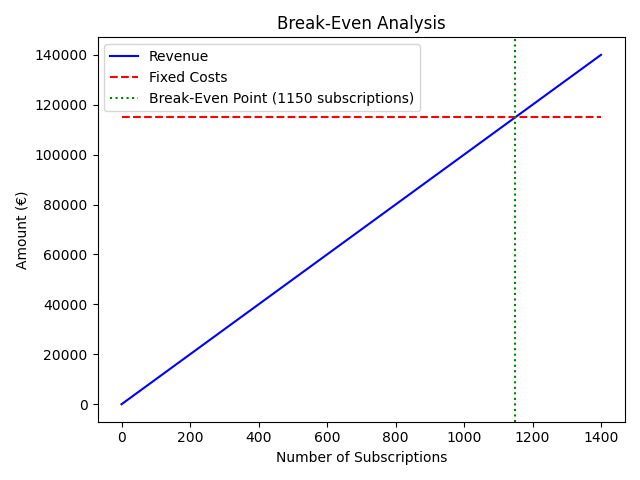
\includegraphics[width=0.8\textwidth]{images/Break Even.png}
    \caption{Expense breakdown showing fixed and variable costs.}
    \label{fig:expense_breakdown}
\end{figure}



\subsection{Conclusion}
By 2027, DynoCharge aims to achieve €12M in revenue and capture a 25\% market share in Europe’s fast-charging segment. Our focus on speed, sustainability, and strategic partnerships positions us to lead the transition to zero-emission mobility.


% Conclusion
% \input{con}

\end{document}